\chapter{Existential Import}\label{ch:existentialimport}
\markright{Ch. \ref{ch:existentialimport}: Existential Import}



\section{Existential Import and Conditionally Valid Forms}

\label{sec:conditionally_valid_forms}
In the last section, we mentioned that you can prove more syllogisms valid if you make different assumptions about existential import. Recall that a statement has existential import if, when you assert the statement, you are also asserting the existence of the things the statement talks about. (See page \pageref{def:Existential_import}.) So if you interpret a mood-A statement as having existential import, it not only asserts ``All $S$ is $P$,'' it also asserts ``There are some $S$.'' or, equivalently, ``Some $S$ exist.'' Thus the mood-A statement ``All unicorns have one horn'' is false, if it is taken to have existential import, because unicorns do not exist. It is probably true, however, if you do not imagine the statement as having existential import. If anything is true of unicorns, it is that they would have one horn if they existed.\footnote{Existence is a complex topic in philosophy, including the truth conditions for evaluating sentences like ``Frodo Baggins is a hobbit.'' or ``Unicorns have one horn.'' See e.g. the Stanford Encyclopedia of Philosophy article on Fictional Entities: \href{https://plato.stanford.edu/entries/fictional-entities/}{https://plato.stanford.edu/entries/fictional-entities/}}

We saw in section \ref{sec:ExistentialImport} that before Boole, Aristotelian thinkers had all sorts of opinions about existential import, or, as they put it, whether a term ``supposits.'' This generally led them to recognize additional syllogism forms as valid. You can see this pretty quickly if you just remember the traditional square of opposition. The traditional square allowed for many more valid immediate inferences than the modern square. It stands to reason that traditional ideas about existential import will also allow for more valid syllogisms.

Our system of Venn diagrams can't represent all of the alternative ideas about existential import. For instance, it has no way of representing Ockham's belief that mood-O statements do \emph{not} have existential import. Nevertheless, it would be nice if we could expand our system of Venn diagrams to show that some syllogisms are valid if you make additional assumptions about existence.

Consider the argument Barbari (AAI-1).

\begin{kormanize}
\premise{All $M$ are $P$.}
\premise{All $S$ are $M$.}
\conclusion{Some $S$ are $P$.}
\end{kormanize}

You won't find this argument in the list of unconditionally valid forms in Table \ref{tab:unconditionally_valid}. This is because under Boolean assumptions about existence it is not valid. The Venn diagram, which follows Boolean assumptions, shows this.


%\begin{figure}
%\centering

%\end{figure}



This is essentially the same argument as Barbara, but the mood-A statement in the conclusion has been replaced by a mood-I statement. We can see from the diagram that the mood-A statement ``All $S$ are $P$'' is true. There is no place to put an $S$ other than in the overlap with $P$. But we don't actually know the mood-I statement ``Some $S$ is $P$,'' because we haven't drawn an x in that spot. Really, all we have shown is that \emph{if} an $S$ existed, it would be $P$.

But by the traditional square of opposition (p. \pageref{fig:traditionalsquare}) we know that the mood-I statement is true. The traditional square, unlike the modern one, allows us to infer the truth of a particular statement given the truth of its corresponding universal statement. This is because the traditional square assumes that the universal statement has existential import. It is really two statements, ``All $S$ is $P$'' and ``Some $S$ exists.''

Because the mood-A statement is actually two statements on the traditional interpretation, we can represent it simply by adding an additional line to our argument. It is always legitimate to change an argument by making additional assumptions. The new argument won't have the exact same impact on the audience as the old argument. The audience will now have to accept an additional premise, but in this case all we are doing is making explicit an assumption that the Aristotelian audience was making anyway. The expanded argument will look like this:

\begin{kormanize}
\premise{All $M$ are $P$.}
\premise{All $S$ are $M$.}
\premise{Some $S$ exists.*}
\conclusion{Some $S$ are $P$}
\end{kormanize}

Here the asterisk indicates that we are looking at an implicit premise that has been made explicit. This is similar to what we did in Chapter \ref{ch:incomplete_arguments} on adding warrants. Now that we have an extra premise, we can add it to our Venn diagram. Since there is only one place for the $S$ to be, we know where to put our x.

%\begin{figure}
%\centering

%\end{figure}



\newglossaryentry{critical term}
{
name=critical term,
description={the term that names things that must exist in order for a conditionally valid argument to be actually valid.}
}

In this argument $S$ is what we call the ``critical term.'' The \textsc{\gls{critical term}}\label{def:critical_term} is the term that names things that must exist in order for a conditionally valid argument to be actually valid. In this argument, the critical term was $S$, but sometimes it will be $M$ or $P$.

We have used Venn diagrams to show that Barbari is valid once you include the additional premise. Using this method we can identify nine more forms, on top of the previous 15, that are valid if we add the right existence assumptions (Table \ref{tab:full_twentyfour})

\begin{table}
\begin{longtabu}{X[1,c] X[1,c] X[1,c] X[1,c] X[1,c]}

\textbf{Figure 1} & \textbf{Figure 2} & \textbf{Figure 3} & \textbf{Figure 4} & \textbf{Condition} \\
\endhead

\multirow{5}{*}{Unconditionally Valid (Boolean Interpretation)}

Barbara (AAA)  & Camestres (AEE) & Disamis (IAI) & Calemes (AEE)  & \\
Celarent (EAE) & Cesare (EAE)    & Bocardo (OAO) & Dimatis (IAI)  & \\
Ferio (EIO)    & Festino (EIO)   & Ferison (EIO) & Fresison (EIO) & \\
Darii (AII)    & Baroco (AOO)    & Datisi (AII)  &                & \\

&&&&\\
\hline
&&&&\\

\multirow{5}{*}{Conditionally Valid (Aristotelian Interpretation)}
Barbari (AAI)   & Camestros (AEO) &                & Calemos (AEO) & $S$ exists \\
Celaront (EAO)  & Cesaro (EAO)    &                &               & $S$ exists \\
                &                 & Felapton (EAO) & Fesapo (EAO)  & $M$ exists \\
                &                 & Darapti (AAI)  &               & $M$ exists \\
                &                 &                & Bamalip (AAI) & $P$ exists \\
\end{longtabu}
\caption{All 24 Valid Syllogisms}
\label{tab:full_twentyfour}
\end{table}

Thus we now have an expanded method for evaluating arguments using Venn diagrams. To evaluate an argument, we first use a Venn diagram to determine whether it is unconditionally valid. If it is, then we are done. If it is not, then we see if adding an existence assumption can make it conditionally valid. If we can add such an assumption, add it to the list of premises and put an x in the relevant part of the Venn diagram. If we cannot make the argument valid by including additional existence assumptions, we say it is completely invalid.

Let's run through a couple examples. Consider the argument EAO-3.

\begin{kormanize}
\premise{No $M$ are $P$.}
\premise{All $M$ are $S$.}
\conclusion{Some $S$ are not $P$.}
\end{kormanize}

First we use the regular Venn digram method to see whether the argument is unconditionally valid.


%\begin{figure}
%\centering

%\end{figure}



We can see from this that the argument is not valid. The conclusion says that some $S$ are not $P$, but we can't tell that from this diagram. There are three possible ways something could be $S$, and we don't know if any of them are occupied.

Simply adding the premise $S$ exists won't help us, because we don't know whether to put the x in the overlap between $S$ and $M$, the overlap between $S$ and $P$, or in the area that is just $S$. Of course, we would want to put it in the overlap between $S$ and $M$, because that would mean that there is an $S$ that is not $P$. However, we can't justifying doing this simply based on the premise that $S$ exists.

The premise that $P$ exists will definitely not help us. The $P$ would either go in the overlap between $S$ and $P$ or in the area that is only $P$. Neither of these would show ``Some $S$ is not $P$.''

The premise ``$M$ exists'' does the trick, however. If an $M$ exists, it has to also be $S$ but not $P$. And this is sufficient so show that some $S$ is not $P$. We can then add this additional premise to the argument to make it valid.

\begin{kormanize}
\premise{No $M$ are $P$.}
\premise{All $M$ are $S$.}
\premise{$M$ exists.*}
\conclusion{Some $S$ are not $P$.}
\end{kormanize}

Checking it against Table \ref{tab:full_twentyfour}, we see that we were right: this is a conditionally valid argument named Felapton.

Now consider the argument EII-3:

\begin{kormanize}
\premise{No $M$ are $P$.}
\premise{Some $M$ are $S$.}
\conclusion{Some $S$ are $P$.}
 \end{kormanize}

First we need to see if it is unconditionally valid. So we draw the Venn diagram.


%\begin{figure}
%\centering

%\end{figure}


The conclusion says that some $S$ are $P$, but we obviously don't know this from the diagram above. There is no x in the overlap between $S$ and $P$. Part of that region is shaded out, but the rest could go either way.

What about conditional validity? Can we add an existence assumption that would make this valid? Well, the x we have already drawn lets us know that both $S$ and $M$ exist, so it won't help to add those premises. What about adding $P$? That won't help either. We could add the premise ``$P$ exists'' but we wouldn't know whether that $P$ is in the overlap between $S$ and $P$ or in the area to the right, which is just $P$.

Therefore this argument is invalid. And when we check the argument against Table \ref{tab:full_twentyfour}, we see that it is not present.

\section{Rules and Fallacies}

\label{sec:rules_and_fallacies}
Did you do the exercises in Part \ref{ex_on_syllogism_patterns} of Section \ref{sec:testing_validity}? If you didn't, go back and think about those questions now, before reading any further. The problem set had five general questions like, ``Can a valid argument have only negative premises?'' The point of those questions was to get you to think about what patterns might exist among the 256 Aristotelian syllogisms, and how those patterns might single out 24 syllogisms as the only ones that can be valid.

In this section, we are going to answer the questions in Part \ref{ex_on_syllogism_patterns} in detail by identifying rules that all valid syllogisms amongst the 256 Aristotelian syllogisms must obey. Seeing these rules will help you understand the \emph{structure} of this part of logic. We aren't just  assigning the labels ``valid'' and ``invalid'' to arguments randomly. Each of the rules we will identify is associated with a fallacy. If you violate the rule, you commit the fallacy.

The fallacies in this section are like the fallacies that are identified in the parts of the in Part \ref{part:CT_and_informal_logic}in that they represent mistakes in reasoning. If you make an inference that commits one of these fallacies, you have used reasoning incorrectly. However, unlike the fallacies we looked at in the Critical Thinking section, many of these fallacies are not even tempting. They are not ways the human mind goes naturally off the rails. They are just things that you shouldn't do.

In the next subsection we are going to outline five basic rules and the fallacies that go with them, along with an addition rule/fallacy pair that can be derived from the initial five. All standard logic textbooks these days use some version of these rules, although they might divide them up differently. Some textbooks also include rules that we have built into our definition of an Aristotelian syllogism in standard form. For instance, other textbooks might have a rule here saying valid syllogisms can't have four terms, or have to use terms in the same way each time. All of this is built into our definitions of an Aristotelian syllogism and standard form for such a syllogism, so we don't need to discuss them here.

\subsection{Six Rules and Fallacies}

\begin{quotation}
\textbf{Rule 1}: The middle term in a valid Aristotelian syllogism must be distributed at least once.
\end{quotation}

\newglossaryentry{fallacy of the undistributed middle}
{
name=fallacy of the undistributed middle,
description={A fallacy committed in an Aristotelian syllogism where the middle term is not distributed in either premise.}
}

Consider these two arguments:

\begin{tabu}{X[1,l] X[1,l]}

\begin{kormanize}
\premise{All $M$ are $P$.}
\premise{All $S$ are $M$.}
\conclusion{All $S$ are $P$.}
\end{kormanize}

&

\begin{kormanize}
\premise{All $P$ are $M$.}
\premise{All $S$ are $M$.}
\conclusion{All $S$ are $P$.}
\end{kormanize}

\end{tabu}

The syllogism on the left (Barbara) is obviously valid, but if you change it to figure 2, you get the syllogism on the right, which is obviously invalid. What causes this change?

The premises in the second syllogism say that $S$ and $P$ are both parts of $M$, but they no longer tell us anything about the relationship between $S$ and $P$. To see why this is the case, we need to bring back a term we saw on page \pageref{def:Distribution}, distribution. A term is distributed in a statement if the statement makes a claim about every member of that class. So in ``All $M$ are $P$'' the term $M$ is distributed, because the statement tells us something about every single $M$. They are all also $P$. The term $P$ is not distributed in this sentence, however. We do not know anything about every single $P$. We know that $M$ is in $P$, but not vice versa.

In general mood-A statements distribute the subject, but not the predicate. This means that when we reverse $P$ and $M$ in the first premise, we create an argument where $S$ and $P$ are distributed, but $M$ is not. This means that the argument is always going to be invalid.

This short argument can show us that arguments with an undistributed middle are always invalid: The conclusion of an Aristotelian syllogism tries to say something about the relationship between $S$ and $P$. It does this using the relationship those two terms have to the third term $M$. But if $M$ is never distributed, then $S$ and $P$ can be different, unrelated parts of $M$. Therefore arguments with an undistributed middle are invalid. Syllogisms that violate this rule are said to commit the \textsc{\gls{fallacy of the undistributed middle}}. \label{def:undistributed_middle}

\begin{quotation}
\begin{tabu}{p{.1\linewidth}p{.9\linewidth}}
\textbf{Rule 2}: & If a term is distributed in the conclusion of a valid Aristotelian syllogism, then it must also be distributed in one of the premises.
\end{tabu}
\end{quotation}

Suppose, instead of changing Barbara from a figure 1 to a figure 2 argument, we changed it to a figure 4 argument. This is what we'd get.

\begin{kormanize}
\premise{All $P$ are $M$.}
\premise{All $M$ are $S$.}
\conclusion{All $S$ are $P$.}
\end{kormanize}

When we changed the argument from figure 1 to figure 2, it ceased to be valid because the middle became undistributed. But this time the middle is distributed in the second premise, and the argument still doesn't work. You can see this by filling in ``animals,'' ``mammals,'' and ``dogs,'' for $S$, $M$, and $P$.

\begin{kormanize}
\premise{All dogs are mammals.    \quad$\Leftarrow$ True}
\premise{All mammals are animals. \quad$\Leftarrow$ True}
\premise{All animals are dogs.    \quad$\Leftarrow$ False}
\end{kormanize}

This version of the argument has true premises and a false conclusion, so you know the argument form must be invalid. \label{counter_example_method_instance} A valid argument form should never be able to take true premises and turn them into a false conclusion. What went wrong here?

The conclusion is a mood-A statement, which means it tries to say something about the entire subject class, namely, that it is completely contained by the predicate class. But that is not what these premises tell us. The premises tell us that the the subject class, animals, is actually the broadest class of the three, containing within it the classes of mammals and dogs.

As with the previous rule, the problem here is a matter of distribution. The conclusion has the subject class distributed. It wants to say something about the entire subject class, animals. But the premises do not have ``animals'' as a distributed class. Premise 1 distributes the class ``dogs'' and premise 2 distributes the class ``mammals.''

Here is another argument that makes a similar mistake:

\begin{kormanize}
\premise{All $M$ are $P$.}
\premise{Some $S$ are not $M$.}
\conclusion{Some $S$ are not $P$.}
\end{kormanize}

This time the conclusion is a mood-O statement, so the predicate term is distributed. We are trying to say something about the entire class $P$. But again, the premises do not say something about the entire class $P$. $P$ is undistributed in the major premise.

\newglossaryentry{fallacy of illicit process}
{
name=fallacy of illicit process,
description={A fallacy committed in an Aristotelian syllogism when a term is distributed in the conclusion but is not distributed in the corresponding premise. This fallacy is called ``illicit major'' or ``illicit minor'' depending on which term is not properly distributed. }
}


These examples illustrate rule 2: If a term is distributed in the conclusion, it must also be distributed in the corresponding premise. Arguments that violate this rule are said to commit the \textsc{\gls{fallacy of illicit process}}. \label{def:illicit_process} This fallacy has two versions, depending on which term is not distributed. If the subject term is the one that is not distributed, we say that the argument commits the fallacy of an illicit minor. If the predicate term isn't distributed, we say that the argument commits the fallacy of the illicit major. Some particularly silly arguments commit both.

The justification for this rule is easy enough to see. If the conclusion makes a claim about all of a class, but the premises only make a claim about some of the class, the conclusion clearly says more than what the premises justify.

\begin{quotation}
\begin{tabu}{p{.1\linewidth}p{.9\linewidth}}
\textbf{Rule 3}: & A valid Aristotelian syllogism cannot have two negative premises.
\end{tabu}\label{rule_3}
\end{quotation}

\newglossaryentry{fallacy of exclusive premises}
{
name=fallacy of exclusive premises,
description={A fallacy committed in an Aristotelian syllogism where both premises are negative.}
}

Back in exercise set \ref{no_conclusion_set1} you were asked to determine what conclusion, if any, could be drawn from a given pair of premises. Some of the exercises involved arguments with two negative premises. Problem \ref{itm:no_conclusion_set1_EEE} went like this: ``No $P$ are $M$, and no $M$ are $S$, therefore \underline{\hspace{2cm}}.'' If you haven't done so already, try to find a conclusion about $S$ and $P$ that you can draw from this pair of premises.

Hopefully you have convinced yourself that there is no conclusion to be drawn  from the premises above using standard Aristotelian format. No matter what mood you put the conclusion is, it will not follow from the premises. The same thing would be true of any syllogism with two negative premises. We could show this conclusively by running through the 16 possible combinations of negative premises and figures. A more intuitive proof of this rule goes like this: The conclusion of an Aristotelian syllogism must tell us about the relationship between subject and predicate. But if both premises are negative then the middle term must be disjoint, either entirely or partially, from the subject and predicate terms. An argument that breaks this rule is said to commit the \textsc{\gls{fallacy of exclusive premises}}. \label{def:exclusive_premises}


\begin{quotation}
\begin{tabu}{p{.1\linewidth}p{.9\linewidth}}
\textbf{Rule 4}: & A valid Aristotelian syllogism can have a negative conclusion if and only if it has exactly one negative premise.
\end{tabu} \label{rule_4}
\end{quotation}
\label{rule4}

\newglossaryentry{negative-affirmative fallacy}
{
name=negative-affirmative  fallacy,
description={A fallacy committed in an Aristotelian syllogism where the conclusion is negative but both of the premises are positive or the conclusion is affirmative but one or more of the premises is negative.}
}

Again, let's start with examples, and try to see what is wrong with them.

\begin{tabu}{p{.5\linewidth}p{.5\linewidth}}

\begin{kormanize}
\premise{All $M$ are $P$.}
\premise{All $P$ are $M$.}
\conclusion{Some $S$ are not $P$.}
\end{kormanize}

&

\begin{kormanize}
\premise{No $P$ are $M$.}
\premise{All $S$ are $M$.}
\conclusion{All $S$ are $P$.}
\end{kormanize}

\end{tabu}

These arguments are so obviously invalid, you might look at them and say, ``Sheesh, is there anything \emph{right} about them?'' Actually, these arguments obey all the rules we have seen so far. Look at the left hand argument. Premise 1 ensures that the middle term is distributed. The conclusion is mood O, which means the predicate is distributed, but $P$ is also distributed in the second premise. The argument does not have two negative premises. A similar check will show that the argument on the right also obeys the first three rules.

Actually, these arguments illustrate an important premise that is independent of the previous three. You can't draw a negative conclusion from two affirmative premises, and you cannot drawn an affirmative conclusion if there is a negative premise. Because the previous rule tells us that you can never have two negative premises, we can actually state this rule quite simply: an argument can have a negative conclusion if and only if it has exactly one negative premise. (The phrase ``if and only if'' will become important when we get to SL in Chapter \ref{ch:SL}. For now you can just note that ``if and only if'' means that the rule goes both ways. If you have a negative conclusion, then you must have one negative premise, and if you have one negative premise, you must have a negative conclusion.)

To see why this rule is justified, you need to look at each part of it separately. First, consider the case with the affirmative conclusion. An affirmative conclusion tells us that some or all of $S$ is contained in $P$. The only way to show this is if some or all of $S$ is in $M$, and some or all of $M$ is in $P$. You need a complete chain of inclusion. Therefore if an argument has a negative premise, it cannot have an affirmative conclusion.

On the other hand, if an argument has a negative conclusion, it is saying that $S$ and $P$ are at least partially separate. But if you have all affirmative premises you are never separating classes. Also, a valid argument cannot have two negative premises. Therefore, a valid argument with a negative conclusion must have exactly one negative premise.

There is not a succinct name for the fallacy that goes with violating this rule, because this is not a mistake people commonly make. We will call it the \textsc{\gls{negative-affirmative fallacy}}. \label{def:negative-affirmative _fallacy}

\begin{quotation}
\begin{tabu}{p{.1\linewidth}p{.9\linewidth}}
\textbf{Rule 5}: & A valid Aristotelian syllogism cannot have two universal premises and a particular conclusion.
\end{tabu} \label{rule_5}
\end{quotation}


\newglossaryentry{existential fallacy}
{
name=existential fallacy,
description={A fallacy committed in an Aristotelian syllogism where the conclusion is particular but both premises are universal. }
}

This rule is a little different than the previous ones, because it really only applies if you take a Boolean approach to existential import. Consider Barbari, the sometimes maligned step-sister of Barbara:

\begin{kormanize}
\premise{All $M$ are $P$.}
\premise{All $S$ are $M$.}
\conclusion{Some $S$ are $P$.}
\end{kormanize}

This syllogism is not part of the core 15 valid syllogisms we identified with the Venn diagram method using Boolean assumptions about existential import. The premises never assert the existence of something, but the conclusion does. And this is something that is generally true under the Boolean interpretation. Universal statements never have existential import and particular statements always do. Therefore you cannot derive a particular statement from two universal statements.

Some textbooks act as if the ancient Aristotelians simply overlooked this rule. They say things like ``the traditional account paid no attention to the problem of existential import'' which is simply false. As we have seen, the Latin part of the Aristotelian tradition engaged in an extensive discussion of the issue from the 12th to the 16th centuries, under the heading ``supposition of terms'' \citep{Read2002}. And at least some people, like William of Ockham, had consistent theories that show why syllogisms like Barbari were valid \citep{Parsons2008}.

In this textbook, we handle the existential import of universal statements by adding a premise, where appropriate, which makes the existence assumption explicit. So Barbari should look like this.

\begin{kormanize}
\premise{All $M$ are $P$.}
\premise{All $S$ are $M$.}
\premise{Some $S$ exist.*}
\conclusion{Some $S$ are $P$.}
\end{kormanize}

Adding this premise merely gives a separate line in the proof for an idea that Ockham said was already contained in premise 2. And if we make it a practice of adding existential premises to arguments like these, Rule 5 still holds true. You cannot conclude a particular statement from all universal premises. However in this case, we do have a particular premise, namely, P$_3$. So if we provide this reasonable accommodation, we can see that syllogisms like Barbari are perfectly good members of the valid syllogism family. We will say, however, that an argument like this that does not provide the extra premise commits the
\textsc{\gls{existential fallacy}}. \label{def:existential_fallacy}


\subsection{Proving the Rules}

For each rule, we have presented an argument that any syllogism that breaks that rule is invalid. It turns out that the reverse is also true. If a syllogism obeys all five of these rules, it must be valid. In other words, these rules are \emph{sufficient} to characterize validity for Aristotelian syllogisms. \nix{(For a discussion of the term ``sufficient'' see page [ref]).} It is good practice to actually walk through a proof that these five rules are sufficient for validity. After all, that sort of proof is what formal logic is really all about. The proof below follows Hurley (\cite*	{Hurley2014}).

Imagine we have a syllogism that obeys the five rules above. We need to show that it must be valid. There are four possibilities to consider: the conclusion is either mood A, mood E, mood I, or mood O.

If the conclusion is in mood A, then we know that $S$ is distributed in the conclusion. If the syllogism obeys rules 1 and 2, then we know that $S$ and $M$ are distributed in the premises. Rule 4 tells us that both premises must be affirmative, so the premises can't be I or O. They can't be E, either, because E does not distribute any terms, and we know that terms are distributed in the premises. Therefore both premises are in mood A. Furthermore, we know that they are in the first figure, because they have to distribute $S$ and $M$. Therefore the syllogism is Barbara, which is valid.

Now suppose the conclusion is in mood E. By rule 4, we have one negative and one affirmative premise. Because mood-E statements distribute both subject and predicate, rules 1 and 2 tell us that all three terms must be distributed in the premises. Therefore one premise must be E, because it will have to distribute two terms. Since E is negative, the other premise must be affirmative, and since it has to distribute a term, it can't be I. So we know one premise is A and the other E. If all the terms are distributed, this leaves us four possibilities: EAE-1, EAE-2, AEE-2, and AEE-4. These are the valid syllogisms Celarent, Cesare, Camestres, and Calemes.

Next up, consider the case where the conclusion is in mood I. By rule 4, it has two affirmative premises, and by rule 5 both premises cannot be universal. This means that one premise must be an affirmative particular statement, that is, mood I. But we also know that by rule 1 some premise must distribute the middle term. Since this can't be the mood-I premise, it must be the other premise, which then must be in mood A. Again we are reduced to four possibilities: AII-1,  AII-2, IAI-3, and IAI-4, which are the valid syllogisms Darii, Datisi, Disamis, and Dimatis.

Finally, we need to consider the case where the conclusion is mood O. Rule 4 tells us that one premise must be negative and the other affirmative, and rule 5 tells us that they can't both be universal. Rules 1 and 2 tell us that $M$ and $P$ are distributed in the premises. This means that the premises can't both be particular, because then one would be I and one would be O, and only one term could be distributed. So one premise must be negative and the other affirmative, and one premise must be particular and the other universal. In other words, our premises must be a pair that goes across the diagonal of the square of opposition, either an A and an O or an E and an I.

With the AO pair, there are two possibilities that distribute the right terms: OAO-3 and AOO-II. These are the valid syllogisms Bocardo and Baroco. With the EI pair, there are four possibilities, which are all valid. They are the EIO sisters: Ferio, Festino, Ferison, and Fresison.

So there you have it. Those five rules completely characterize the possible valid Aristotelian syllogisms. Any other patterns you might notice among the valid syllogisms can be derived from these five rules. For instance, Problem \ref{itm:two_particulars} in exercise set \ref{ex_on_syllogism_patterns} of Section \ref{sec:testing_validity} asked if you could have a valid Aristotelian syllogism with two particular premises. If you did that problem, hopefully you saw that the answer was ``no.'' We could, in fact, make this one of our five rules above. But we don't need to. When we showed that these five rules were sufficient to characterize validity, we also showed that any other rule characterizing validity that we care to come up with can be derived from the rules we already set out. So, let's state the idea that a syllogism cannot have two particular premises as a rule, and show how it can be derived. This will be our statement of the rule:

 \begin{quotation}
\begin{tabu}{p{.25\linewidth}p{.75\linewidth}}
\textbf{Derived Rule 1}: &  A valid Aristotelian syllogism cannot have two particular premises.
\end{tabu}\label{derived_rule_1}
\end{quotation}

\newglossaryentry{fallacy of particular premises}
{
name=fallacy of particular premises,
description={A fallacy committed in an Aristotelian syllogism where both premises are particular.}
}

And let's call the associated fallacy the \textsc{\gls{fallacy of particular premises}}. \label{def:particular_premises} To show that this rule can be derived from the previous five, it is sufficient to show that any syllogism that violates this rule will also violate one of the previous five rules. Thus there will always be a reason, independent of this rule, that can explain why that syllogism is false.

So suppose we have a syllogism with two particular premises. If we want to avoid violating rule 1, we need to distribute the middle term, which means that both premises cannot be mood I, because mood-I statements don't distribute any term. We also know that both statements can't be mood O, because rule 3 says we can't have two negative premises. Therefore our syllogism has one premise that is I and one premise that is O. It thus has exactly one negative premise, and by rule 4, must have a negative conclusion, either an E or an O. But an argument with premises I and O can only have one term distributed: if the conclusion is mood O, then two terms are distributed; and if it is mood E then all three terms are distributed. Thus any syllogism that manages to avoid rules 1, 3, and 4 will fall victim to rule 2. Therefore any syllogism with two particular premises will violate one of the five basic rules.

\section{Validity and the Counterexample Method}
\label{sec:counterexample}

Except for a brief discussion of logically structured English in section \ref{sec:form_mood_figure}, so far, we have only been evaluating arguments that use variables for the subject, middle, and predicate terms. Now, we will be looking in detail at issues that come up when we try to evaluate categorical arguments that come up in ordinary English. In this section we will consider how your knowledge of the real world terms discussed in an argument can distract you from evaluating the form of the argument itself. In this section we will consider difficulties in putting ordinary language arguments into logically structured English, so they can be analyzed using the techniques we have learned.

Let's go back again to the definition of validity on page \pageref{def:valid}. (It is always good for beginning student to reinforce their understanding of validity). We did this in the last chapter in Section \ref{sec:ESA}, and we are doing it again now. \label{valid_definition_reinforcement} Validity is a fundamental concept in logic that can be confusing. A valid argument is not necessarily one with true premises or a true conclusion. An argument is valid if the premises \emph{would} make the conclusion true \emph{if} the premises were true.

This means that, as we have seen before, there can be valid arguments with false conclusions. Consider this argument:

\begin{quotation}\noindent No reptiles are chihuahuas. But all dogs are reptiles. Therefore, no dogs are chihuahuas. \end{quotation}

This seems silly, if only because the conclusion is false. We know that some dogs are chihuahuas. But the argument is still valid. In fact, it shares a form with an argument that makes perfect sense:

\begin{quotation}\noindent No reptiles are dogs, but all chameleons are reptiles. Therefore, no dogs are chameleons. \end{quotation}

Both of these arguments have the form Celarent:

\begin{kormanize}
\premise{No $M$ are $P$.}
\premise{All $S$ are $M$.}
\conclusion{ No $S$ are $P$.}
\end{kormanize}

This form is valid, whether the subject and predicate term are dogs and chameleons, or dogs and chihuahuas, which you can see from this Venn diagram.

%\begin{figure}
%\centering
%\begin{syllogism}
%\end{syllogism}
%\end{figure}


This means you can't assume an argument is invalid because it has a false conclusion. The reverse is also true. You can't assume an argument is valid just because it has a true conclusion. Consider this

\begin{quotation}  All cats are animals, and some animals are dogs. Therefore no dogs are cats. \end{quotation}

Makes sense, right? Everything is true. But the argument isn't valid. The premises aren't making the conclusion true. Other arguments with the same form have true premises and a false conclusion. Like this one.

\begin{quotation}All chihuahuas are animals, and some animals are dogs. Therefore, no dogs are chihuahuas.\end{quotation}

Really, the arguments in both these passages have the same form: AEE-IV:

\begin{kormanize}
\premise{All $P$ are $M$.}
\premise{Some $M$ are $S$.}
\conclusion{No $S$ are $P$.}
\end{kormanize}

This in an invalid form, and it remains invalid whether the $P$ stands for cats or chihuahuas. You can see this in the Venn diagram:

%\begin{figure}
%\centering
%\begin{syllogism}
%\end{syllogism}
%\end{figure}


All these examples bring out an important fact about the kind of logic we are doing in this chapter and the last one: this is \emph{formal} logic. As we discussed on page \pageref{def:Formal_logic} formal logic is a way of making our investigation content neutral. By using variables for terms instead of noun phrases in English we can show that certain ways of arguing are good or bad regardless of the topic being argued about. This method will be extended in Chapters \ref{ch:SL} and \ref{ch:QL}, when we introduce our full formal languages SL and QL.
This method will be extended in Part \ref{part:sent_logic}, when we introduce the full formal language SL.


The examples above also show us another way of proving that an argument given in English is invalid, called the counterexample method. As we have just seen, if you are given an argument in English with, say, false premises and a false conclusion, you cannot determine immediately whether the argument is valid. However, we can look at arguments that have the same form, and use them to see whether the argument is valid. If we can find an argument that has the exact same form as a given argument but has true premises and a false conclusion, then we know the argument is invalid. We just did that with the AEE-IV argument above. We were given an argument with true premises and a true conclusion involving cats, dogs, and animals. We were able to show this argument invalid by finding an argument with the same form that has true premises and a false conclusion, this time involving chihuahuas, dogs, and animals.


\newglossaryentry{counterexample method}
{
name=counterexample method,
description={A method for determining whether an argument with ordinary English words for terms is valid. One consistently substitutes other English terms for the terms in the given argument to see whether one can find an argument with the same form that has true premises and a false conclusion.}
}

More precisely, we can define the \textsc{\gls{counterexample method}} \label{def:counter_example_method} as a method for determining if an argument with ordinary English words for terms is valid, where one consistently substitutes other English terms for the terms in the given argument to see if one can find an argument with the same form that has true premises and a false conclusion. Let's run through a couple more examples to see how this works.

First consider this argument in English:

\begin{quotation}
\noindent  All tablet computers are computers. We know this because a computer is a kind of machine, and some machines are not tablet computers.
\end{quotation}

Every statement in this argument is true, but it doesn't seem right. The premises don't really relate to the conclusion. That means you can probably find an argument with the same form that has true premises and a false conclusion. Let's start by putting the argument in canonical form. Notice that the English passage had the conclusion first.

\begin{kormanize}
\premise{All computers are machines.}
\premise{Some machines are not tablet computers.}
\conclusion{All tablet computers are computers.}
\end{kormanize}

Let's find substitutes for ``machines,'' ``computers,'' and ``tablet computers'' that will give us true premises and a false conclusion. It is easiest to work with really common sense categories, like ``dog'' and ``cat.'' It is also easiest to start with a false conclusion and then try to find a middle term that will give you true premises. ``All dogs are cats'' is a nice false conclusion to start with:

\begin{kormanize}
\premise{All cats are $M$.}
\premise{Some $M$ are not dogs.}
\conclusion{All dogs are cats.}
 \end{kormanize}

So what can we substitute for $M$ (which used to be ``machines'') that will make P$_1$ and P$_2$ true? ``Animals'' works fine.

\begin{kormanize}
\premise{All cats are animals.}
\premise{Some animals are not dogs.}
\conclusion{All dogs are cats.}
 \end{kormanize}

There you have it: a counterexample that shows the argument invalid. Let's try another one.

\begin{quotation}
Some diseases are viral, therefore some things caused by bacteria are not things that are caused by viruses, because all diseases are bacterial.
\end{quotation}

This will take a bit more unpacking. You can see from the indicator words that the conclusion is in the middle. We also have to fix ``viral'' and ``things that are caused by viruses'' so they match, and the same is true for ``bacterial'' and ``things that are caused by bacteria.'' Once we have the sentences in canonical form, the argument will look like this:

\begin{kormanize}
\premise{Some diseases are things caused by viruses.}
\premise{All diseases are things causes by bacteria.}
\conclusion{Some things caused by bacteria are not things caused by viruses.}
\end{kormanize}

Once you manage to think through the complicated wording here, you can see that P$_1$ and the conclusion are true. Some diseases come from viruses, and not everything that comes from a bacteria comes from a virus. But P$_2$ is false. All diseases are not caused by bacteria. In fact, P$_1$ contradicts P$_2$. But none of this is enough to show the argument is invalid. To do that, we need to find an argument with the same form that has true premises and a false conclusion.

Let's go back to the simple categories: ``dogs,'' ``animals,'' etc. We need a false conclusion. Let's go with ``Some dogs are not animals.''

\begin{kormanize}
\premise{Some $M$ are dogs.}
\premise{All $M$ are animals.}
\conclusion{Some dogs are not animals.}
 \end{kormanize}

We need a middle term that will make the premises true. It needs to be a class that is more general than ``dogs'' but more narrow than ``animals.'' ``Mammals'' is a good standby here.

\begin{kormanize}
\premise{Some mammals are dogs.}
\premise{All mammals are animals.}
\conclusion{Some dogs are not animals.}
 \end{kormanize}

And again we have it, a counterexample to the given syllogism.

\section{Ordinary Language Arguments}

In the last section we saw that arguments in ordinary language can throw us off because our knowledge of the truth or falsity of the statements in them can cloud our perception of the validity of the argument. Now we are going to look at ways we might need to transform ordinary language arguments in order to put them in standard form (see p. \pageref{standard_form_for_an_Aristotelian_syllogism}) and use our evaluative tools.

\subsection{Basic Transformations into Logically Structured English}

Arguments are composed of statements, so all of the guidelines we discussed for putting ordinary English statements into logically structured English in Section \ref{sec:transformation} apply here. Also, as you saw in the exercises in Section \ref{sec:form_mood_figure}, we need to be aware that the conclusion of an ordinary language argument can occur anywhere in the passage. Consider this argument

\begin{quotation}
\noindent Every single penguin in the world is a bird. Therefore, at least one bird in the world is not a person, because not one person is a penguin.
\end{quotation}

The indicator words let us know the conclusion is the sentence in the middle of this passage, ``At least one bird in the world is not a person.'' The quantifier in this sentence is nonstandard. As we saw on page \pageref{subsec:nonstandard_quantifiers} ``at least one'' should be changed to ``some.'' That would give us ``Some birds are not people'' for the conclusion. Similar changes need to be made to the two premises. Thus the argument and translation key look like this:

\begin{tabu}{{X[1,l] X[1,l]}}
\begin{description}
\item[$S$:] Birds
\item[$M$:] Penguins
\item[$P$:] People
\end{description}
&
\begin{kormanize}
\premise{No $P$ are $M$.}
\premise{All $M$ are $S$.}
\conclusion{Some $S$ are not $P$.}
\end{kormanize}
\end{tabu}

Now that we have it in this form, we can see that it is the argument Fesapo (EAO-4), which is valid if you add the premise that some penguins exist.

Another issue that can come up in ordinary language arguments is the use of synonyms. Consider another argument about penguins:

\begin{quotation}
\noindent No Ad\'{e}lie penguins can fly, because all members of \emph{Pygoscelis adeliae} are members of the family Sphenisciformes, and no Sphenisciformes can fly.
\end{quotation}

You might think this argument can't be a proper syllogism, because it has four terms in it: Ad\'{e}lie penguins, \emph{Pygoscelis adeliae}, Sphenisciformes, and things that can fly. However, a quick trip to Wikipedia can confirm that \emph{Pygoscelis adeliae} is just the scientific name from the Ad\'{e}lie penguin, and for that matter ``Sphenisciformes'' are just penguins. So really, the argument just has three terms, and there is no problem representing the argument  like this:

\begin{tabu}{{X[1,l] X[1,l]}}
\begin{description}
\item[$S$:] Ad\'{e}lie penguins
\item[$M$:] Penguins
\item[$P$:] Things that can fly
\end{description}
&
\begin{kormanize}
\premise{No $M$ are $P$.}
\premise{All $S$ are $M$.}
\conclusion{No $S$ are $P$.}
\end{kormanize}
\end{tabu}

And this is our good friend Celarent (EAE-1).

Generally speaking, arguments involving different names for the same person can work the same way as synonyms. Consider this argument:

\begin{quotation}
\noindent Bertrand Russell was a philosopher. We know this because Mr. Russell was a logician, and all logicians are philosophers.
\end{quotation}

``Bertrand Russell'' and ``Mr. Russell'' are names for the same person, so we can represent them using the same variable. Back on page \pageref{subsec:singular_propositions} we learned that names for individuals need to be transformed into classes using phrases like ``objects identical with \ldots'' or ``people identical with \ldots.''  Thus the argument turns out to be Celarent's best friend, Barbara (AAA-I):

\begin{tabu}{{X[1.25,l] X[1,l]}}
\begin{description}
\item[$S$:] People identical with Bertrand Russell
\item[$M$:] Logicians
\item[$P$:] Philosophers
\end{description}
&
\begin{kormanize}
\premise{All $M$ are $P$.}
\premise{All $S$ are $M$.}
\conclusion{All $S$ are $P$.}
\end{kormanize}
\end{tabu}

Merging proper nouns into one variable doesn't always work the way merging synonyms does, however. Sometimes exchanging one name with another can change the truth value of a sentence, even when the two names refer to the same person. Any comic book fan will tell you that the sentence ``J. Jonah Jameson hates Spider-Man'' is true. Also, ``Peter Parker'' and ``Spider-Man'' refer to the same person. However ``J. Jonah Jameson hates Peter Parker'' is false. These situations are called ``intentional contexts.'' We won't be dealing with them in this textbook, but you should be aware that they exist.

Another thing to be aware of when you assign variables to terms is that often you will need to find the right general category that will allow your terms to hook up with each other. \label{finding_general_terms} Consider this argument.

\begin{quotation}
Bertrand Russell did not believe in God. I know this because Mr. Russell was not a Christian, and all Christians believe in God
\end{quotation}

Here again we need to use one variable for both ``Bertrand Russell'' and ``Mr. Russell.'' But we also have to change the verb phrase ``believes in God'' into a predicate term (see page \pageref{subsec:nonstandard_verbs}). The main trick here is to transform the verb phrase ``believes in God'' and the singular terms referring to Bertrand Russell in a way that will match. The trick is to use the word ``people'' each time. ``Believes in God'' becomes ``people who believe in God,'' and the two names for Bertrand Russell need to become ``people identical with Bertrand Russell.'' By including the word ``people'' in each case, we ensure that the terms will be comparable.

\begin{tabu}{{X[2,l]X[1,l]}}
\begin{description}
\item[$S$:] People identical to Bertrand Russell
\item[$M$:] Christians
\item[$P$:] People who believe in God
\end{description}
&
\begin{kormanize}
\premise{All $M$ are $P$.}
\premise{No $S$ are $M$.}
\conclusion{No $S$ are $P$.}
\end{kormanize}
\end{tabu}

The argument here is AEE-1, which is invalid. It violates rule 2, because $P$ is distributed in the conclusion, but not the premises. More informally, we can say that just because Russell wasn't a Christian doesn't mean he was an atheist or an agnostic. (In fact, Russell said that he was an atheist in some ways, and an agnostic in others, but this argument doesn't show that.)

\subsection{Complement Classes, Obversion, and Contraposition}

In the last subsection, we saw that we can represent synonyms using the same variable, thus reducing the number of terms in an argument down to the three terms required for an Aristotelian syllogism. Something similar can be done when you have terms that are complements of other terms. Back on page \pageref{def:Complement} we said that the complement of a class was the class of things that are not in the original class. So the complement of the class ``penguins'' is everything that is not a penguin. Sometimes, if you have an argument with more than three terms, you can reduce the number of terms down to three, because some of the terms are complements of each other, like ``penguins'' and ``non-penguins.''

Consider the following argument, which talks about the stoics, an ancient philosophical school and pioneers in logical thinking.

\begin{quotation}
No stoics are non-logicians, and all non-philosophers are non-stoics. Therefore all logicians are philosophers.
\end{quotation}

This argument has six terms: stoics, logicians, philosophers, non-stoics, non-logicians, and non-philosophers. Since the second three are all complements of the first, we should be able to reduce the number of terms to three. Once we do this, we might find that the argument is valid---it looks like it might be Barbara. We can begin by assigning $S$, $M$, and $P$ to the terms ``stoics,'' ``logicians,'' and ``philosophers.'' We can then represent the other six terms as non-$S$, non-$M$, and non-$P$.


\begin{tabu}{{X[1,l]X[1,l]}}

\begin{description}
\item[$S$:] Logicians
\item[$M$:] Stoics
\item[$P$:] Philosophers
\end{description}

&

\begin{kormanize}
\premise{No $M$ are non-$P$.}
\premise{All non-$S$ are non-$M$.}
\conclusion{All $S$ are $P$.}
\end{kormanize}

\end{tabu}

The argument still has six terms, so we can't evaluate it as is. However, we can get rid of three of these terms. The secret is to apply two of the transformation tools we learned about in Section \ref{sec:conv_obv_cont}, obversion and contraposition. In that section, we saw that there were different ways you could alter categorical statements that would sometimes yield a logically equivalent statement. Two of those methods---obversion and contraposition---involved taking the complements of existing terms. In the cases where these transformations yield logically equivalent terms, we can use them to change the premises of an argument into statements that lack the terms we want to get rid of.

In obversion, you change the quality of a sentence---switch it from affirmative to negative or vice versa---and then replace the predicate term with its complement. This process always yields a logically equivalent statement, so we can always use it. Applying obversion to the first premise of the argument above allows us to eliminate the term non-$P$.

\begin{kormanize}
\premise{All $M$ are $P$.}
\premise{All non-$S$ are non-$M$.}
\conclusion{All $S$ are $P$.}
\end{kormanize}

We can also use contraposition to eliminate terms, but here we must be more careful. Contraposition only yields logically equivalent statements when it is applied to mood-A or mood-O statements. Fortunately, Premise 2 is a mood-A statement, so we can change the argument to look like this:

\begin{kormanize}
\premise{All $M$ are $P$.}
\premise{All $M$ are $S$.}
\conclusion{All $S$ are $P$.}
\end{kormanize}

And now the argument only has three terms, and we can evaluate it. As you can see it is not Barbara at all, but one of her unnamed evil step-sisters, AAA-3. Again, remember not to use contraposition on mood-E or mood-I statements. You can use obversion on any statement, but contraposition only works on mood A or mood O.

Ordinary English has other prefixes besides ``non-'' to denote the complements of classes. ``Un-'' is the most common prefix, but English also uses ``in-,'' ``dis-,'' and ``a-.'' These can be handled the same way ``non-'' is. Consider,

\begin{quotation}
All dogs in the park must be leashed. Some unleashed pets in the park are cats. Therefore, some cats in the park are not dogs.
\end{quotation}

To make this argument work, we need to get the predicate of the major premise to match the subject of the minor premise. The first step is just turning the verb phrase ``must be leashed'' into a noun phrase that matches ``unleashed pets.'' We also should use the qualification ``in the park'' consistently across the terms.

\begin{tabu}{{X[1,l] X[1,l]}}

\begin{description}
\item[$S$:] Cats in the park
\item[$M$:] Leashed pets in the park
\item[$P$:] Dogs in the park
\end{description}

&

\begin{kormanize}
\premise{All $P$ are $M$.}
\premise{Some non-$M$ are $S$.}
\conclusion{Some $S$ are not $P$.}
\end{kormanize}

\end{tabu}

Now the trick is to get the terms $M$ and non-$M$ to match. We could try to transform the second premise, but that won't do us any good. It is an E statement, so we can't use contraposition, and obversion won't change the subject term.

Instead of changing the ``non-$M$'' to ``$M$'' in the second premise, we need to change the ``$M$'' to ``non-$M$'' in the first premise. We can do this using obversion, which works on statements in any mood.

\begin{kormanize}
\premise{No $P$ are non-$M$.}
\premise{Some non-$M$ are $S$.}
\conclusion{Some $S$ are not $P$.}
\end{kormanize}

And now we can see that the argument is Fresison (EIO-4), which is valid.


\section{Enthymemes}
\label{sec:enthymemes}
\newglossaryentry{enthymeme}
{
name=enthymeme,
description={An argument where a premise or conclusion has been left unstated.}
}


In the real world, arguments are often presented with pieces missing. The missing piece could be an important premise or sometimes even the conclusion.  Arguments with parts missing are called \textsc{\glspl{enthymeme}}. \label{def:enthymeme} We discuss them extensively in the chapter on incomplete arguments in the full version of this text. Here we will be dealing with them specifically as they are used with Aristotelian syllogisms. Because we are now dealing with more real-world arguments, we will return to our practice of giving the context in italics before passages (see page \pageref{context_marker}). Remember, that this context is not a part of the argument. It is just there to help interpret the passage.

The simplest and most common reason one might leave out a part of an Aristotelian syllogism is brevity. Sometimes part of an argument is common knowledge or completely obvious from the context and simply doesn't need to be said. Consider this common inference that might pop into your head one afternoon:

\begin{quotation} \noindent \textit{Susan is working from home} Well, the dog is barking. I guess that means the mail is here.\end{quotation}

Here the missing premise is that dogs bark at letter carriers. But this isn't something Susan is going to think of consciously. It is completely common knowledge, and probably something Susan has a lot of first-hand experience with as a dog owner. So the passage above basically represents Susan's inference as it occurs to her.

If in order to evaluate the argument, though, we need to make all of the reasoning explicit. This means putting the whole thing in standard form and then finding the missing premise. Once you do that, it becomes clear that this common, everyday inference is actually very complicated. The simplest way to put the argument in canonical form would simply be this:

\begin{kormanize}
\premise{The dog is barking.}
\conclusion{The mail is here.}
\end{kormanize}

But if we are going to use the tools of Aristotelian logic to show that this is valid, we are going to need to convert these statements into categorical statements. The ``now'' functions here as a singular term, so we needed to use the awkward ``times identical with'' construction (see page \pageref{subsec:singular_propositions}). Also, we needed to find a general category to put things under, in this case ``times,'' to be sure that all the terms matched. (This is similar to the ``persons identical to Bertrand Russell example on page \pageref{finding_general_terms}.)

\begin{kormanize}
\premise{All times identical with now are times when the dog is barking.}
\conclusion{All times identical with now are times when the mail arrives.}
\end{kormanize}

Once we do this, we can see that the conclusion is a statement in mood A. The minor term is ``times identical with now'' and the major term is ``times when the mail arrives.'' The premise is a minor premise, because it has the minor term in it, and the middle term is ``times when the dog is barking.'' From this we can see that the missing premise is the major premise. When we add it, the full argument looks like this:

\begin{kormanize}
\premise{All times when the dog is barking are times when the mail arrives*}
\premise{All times identical with now are times when the dog is barking.}
\conclusion{All times identical with now are times when the mail arrives.}
\end{kormanize}

Remember that the asterisks means that an implicit premise has been made explicit. (See Chapter \ref{ch:incomplete_arguments}) Once we have that in place, however, we can see that this argument is just a version of Barbara (AAA-1). The full argument is quite wordy, which shows how much sophisticated reasoning is going on in your brain when you make even the most everyday of inferences.

Enthymemes can also be used to hide premises that are needed for the argument, but that the audience might not accept if their attention were drawn to them. Consider this argument:

\begin{quotation}\noindent \textit{A used car salesperson is showing you a Porsche Cayenne Hybrid SUV} And it is a hybrid electric car, so you know it gets good gas mileage. \end{quotation}

Here again we have an argument about a singular object---this car the salesperson is showing you. So when we represent the argument, we need to use the awkward ``things identical with'' construction.

\begin{kormanize}
\premise{All things identical with this vehicle are hybrid electric vehicles.}
\conclusion{All things identical with this vehicle are vehicles that get good gas mileage.}
\end{kormanize}

Again, we have two mood-A statements. The minor term is ``things identical with this vehicle,'' the middle term is ``hybrid electric vehicles'' and the major term is ``vehicles that get good gas mileage.'' The missing premise must be the major premise ``All hybrid electric vehicles get good gas mileage.''

\begin{kormanize}
\premise{All hybrid electric vehicles are vehicles that get good gas mileage.*}
\premise{All things identical with this vehicle are hybrid electric vehicles.}
\conclusion{All things identical with this vehicle are vehicles that get good gas mileage.}
\end{kormanize}

But wait, is this implicit premise even true? Actually it isn't---the Cayenne itself only gets 20 miles per gallon in the city and 24 on the highway---no wonder the salesperson kept this premise implicit! Compare the Cayenne's mileage to that of a regular gas-powered car like the Honda Fit, which gets 33 city and 41 highway. It is true that hybrids generally get better mileage than similarly sized cars that run on gasoline only, but that isn't the reasoning the salesperson is presenting here. Someone who was really all that concerned about mileage probably should not be in the market for a luxury SUV like the Cayenne.

When filling in missing parts of an enthymeme it is important to remember the principle of charity. The principle of charity says that we should try to interpret other people in a way that makes reasoning coherent and their beliefs reasonable. (See Chapter \ref{ch:incomplete_arguments}.) With the example of the salesperson above, one might argue that we were not being as charitable as we could have been. Perhaps the salesperson didn't expect us to believe that \textit{all} hybrids get good gas mileage. Perhaps they only expected us to believe that \textit{most} hybrids get good gas mileage.

If you interpret the argument this way, you are getting a more believable premise in exchange for a weaker inference. The original argument had the strongest possible inference---it was genuinely valid. If you change the major premise to something involving ``most,'' you will have an argument that is at best strong, not  valid. The premise is now believable, but the inference is fallible.  (This kind of trade-off is discussed more extensively in Chapter \ref{ch:incomplete_arguments}) Also note that if you do decide to use ``most'' when filling in the missing premise, the argument becomes inductive, and thus is something that you would evaluate using the tools from the parts of this textbook on inductive and scientific reasoning, not the tools of Aristotelian logic. In this section we will only be looking at enthymemes where you fill in premises in a way that yields Aristotelian syllogisms.

Sometimes enthymemes are missing a conclusion, rather than a premise. Consider this example:

\begin{tabu}{p{.1\linewidth}p{.7\linewidth}}
\multicolumn{2}{p{.8\linewidth}}{\textit{Annabeth, age 7, is pestering her mother Susan with strange questions.}}\\
\textbf{Annabeth}: & Mommy, do any dogs have forked tongues? \\
\textbf{Susan}:  & Well, dear, all dogs are mammals, and no mammals have forked tongues. So do you think any dogs have forked tongues?\\
\end{tabu}

Teachers and parents often replace the conclusion with a rhetorical question like this because it forces the audience to fill in the missing conclusion for themselves. The effect is going to be different for different audiences, however. A child might be pleased with herself for figuring out the answer with just a few hints. Often replacing the conclusion with a rhetorical question when talking to an adult can be demeaning, for instance, when someone glibly says ``you do the math,'' even when there is no math involved in the issue.

In any case, the proper conclusion for the argument above is ``No dogs have forked tongues.'' The argument is Celarent (EAE-1), and in canonical form it looks like this:

\begin{kormanize}
\premise{No mammals have forked tongues.}
\premise{All dogs are mammals.}
\conclusion{No dogs have forked tongues.}
\end{kormanize}


Evaluating an enthymeme requires four steps. First, you need to figure out if the missing statement is a premise or a conclusion. As you might expect, indicator phrases will be helpful here. Words like ``because'' or ``therefore'' will mark one of the sentences you are given as a premise or a conclusion, and you can use this information to determine what hasn't been given. In fact, if the enthymeme contains any indicator words at all, you can be pretty confident that the missing statement is a premise. If the enthymeme contains a conclusion indicator word like ``therefore,'' you know that the statement after it is the conclusion. But even if the indicator word is a premise indicator word, you the missing statement is still likely to be a premise, because the premise indicator words are generally preceded by conclusions. Consider this following argument.

\begin{quotation} \noindent\textit{Susan is now wondering about what reptilian characteristics some mammals do have} Well, I know some mammals have scales, because armadillos have scales. \end{quotation}

 Here the ``because'' lets us know that  ``Armadillos have scales'' is a premise, and ``some mammals have scales'' is the conclusion. Thus the missing statement is one of the premises.

Once you have figured out what part of the syllogism is missing, the second step is to write the parts of the syllogism you do have in standard form. For this example, that is pretty easy, but you do need to provide the missing quantifier for the premise.

\begin{kormanize}
\premise{All armadillos have scales.}
\conclusion{Some mammals have scales.}
\end{kormanize}

 Step three is to figure out what terms are in the missing statements. The two statements you have been given will contain a total of three terms, one of which will be repeated once in each statement. Since every term in an Aristotelian syllogism appears twice, we know that the two terms that only appear once must be the ones that appear in the missing statement. In the example above, the terms are ``mammals,'' ``armadillos,'' and ``things with scales.'' The term ``things with scales'' is the one that appears twice. So the missing statement will use the terms ``armadillos'' and ``mammals.''

Step four is to determine the mood of the missing statement and the overall figure of the syllogism. This will let you fill in everything else you need to know to complete the syllogism. The rules for a valid syllogism listed in Section \ref{sec:rules_and_fallacies} can be a big help here.

In the example we have been working with we know that the conclusion is ``Some mammals have scales.'' This means that the major term is ``things with scales'' and the minor term is ``mammals.'' The premise that we are given, ``All armadillos have scales'' must then be the major premise. So we know this much:

\begin{kormanize}
\premise{All armadillos have scales.}
\premise{[something with armadillos and mammals]}
\conclusion{Some mammals have scales.}
\end{kormanize}

We also know that the middle term is in the subject position of the major premise, which means that the whole syllogism is either figure 1 or figure 3. Because the major premise and the conclusion are both affirmative, we know by Rule 4 (page \pageref{rule4}) that the minor premise must be affirmative. That leaves us only mood-A and mood-I statements. \label{rule_use}

So there are four possibilities remaining: the argument is either AAI-1, AII-1, AAI-3 or AII-3. A quick glance at the Table \ref{tab:full_twentyfour} tells us that all of these are valid. (Although AAI-1 and AAI-3 are conditionally valid.) So any of these are correct answers. Let's go with AII-1 (Darii):


\begin{kormanize}
\premise{All armadillos have scales}
\premise{Some mammals are armadillos.}
\conclusion{Some mammals have scales.}
\end{kormanize}

Sometimes, when people give enthymemes, there is no way to fill in the missing premise that will make the argument valid. This can happen either because the person making the argument is confused or because they are being deceptive. Let's look at one example:

\begin{quotation}\noindent\textit{Now Annabeth wants a pet armadillo} If an animal makes a good pet, then it must be cute. So armadillos must make good pets. \end{quotation}

There is no way to fill in Annabeth's reasoning here that can turn this into a valid syllogism. To see this, we need to first put it in standard form, which means converting the conditional ``if...then'' statement into a mood-A statement.


\begin{kormanize}
\premise{All animals that make good pets are animals that are cute.}
\conclusion{All armadillos are animals that make good pets.}
\end{kormanize}

It seems like the missing premise here should be ``All armadillos are cute,''  but adding that premise doesn't give us a valid argument.

\begin{kormanize}
\premise{All animals that make good pets are animals that are cute.}
\premise{All armadillos are animals that are cute.}
\conclusion{All armadillos are animals that make good pets.}
\end{kormanize}

The argument is AAA-2, which has an undistributed middle. In fact, there is no way to get from P$_1$ to the conclusion with an Aristotelian categorical statement. The major term has the premise in the subject position, which means that the argument can only be figure 2 or 4. But a quick look at Table \ref{tab:full_twentyfour} lets us know that the only valid argument with a mood-A major premise and a mood-A conclusion is Barbara, which is figure 1. Nice try, kid.

In other cases, the rules given in Section \ref{sec:rules_and_fallacies} can be used to determine whether an enthymeme with a missing conclusion can be valid. In the argument showing that some mammals have scales (p. \pageref{rule_use}), we used Rule 4 to show that the missing premise had to be affirmative. In an enthymeme with a missing conclusion, you might note that there are two negative premises, so that there actually is no valid conclusion to draw. In other situations you might be able to determine that the missing conclusion must be negative. The rules for valid syllogisms are your friends when working with enthymemes, because they allow you to consider broad categories of syllogisms, rather than having to work on a trial and error basis with the Venn diagram method.

% *******************************************
% *                      Sorites Categorical Arguments      *
% *******************************************

\section{Sorites Categorical Arguments }

The Aristotelian tradition mostly focused on syllogisms with two premises; however, there are fun things we can do with longer arguments. These were explored, among other places, in a 19th century textbook called \textit{Symbolic Logic} \citep{Dodgson1896}, by the mathematician and logician Charles Lutwidge Dodgson. (Dodgson is actually better known by his pen name, Lewis Carroll, under which he wrote the children's classics \textit{Alice's Adventures in Wonderland} and \textit{Through the Looking Glass}.)

\newglossaryentry{sorites categorical argument}
{
name=sorites categorical argument,
description={A categorical argument with more than two premises.}
}

Categorical arguments with more than two premises are called \textsc{\glspl{sorites categorical argument}}, \label{def:sorites_categorical_arguments} or just ``Sorites'' (pronounced ``sore-EYE-tease'') for short. The name comes from the Greek word ``Soros'' meaning ``heap.'' This kind of sorites should not be confused with the sorites paradoxes we talk about in the chapter on real world evaluation in the complete version of this text, \label{ver_var} \nix{Chapter \ref{ch:realworldevaluation},} which were arguments that exploited vague premises.

Here is a simple example of a categorical sorites.

\begin{kormanize}
\premise{All carrots are vegetables.}
\premise{No vegetables are houses.} %No carrots are houses
\premise{All houses are buildings.}
\conclusion{No carrots are buildings.}
\end{kormanize}
%Calemes-Celarent

We have more premises and terms than we do in the classic Aristotelian syllogism, but they are arranged in a way that is a natural extension of the Aristotelian syllogism. Every term appears twice, except for the major and minor terms of the conclusion. Each premise shares one term with each of the other premises. Really, this is just like a regular Aristotelian syllogism with more middle terms.

Because the form of the argument above is an extension of the standard form of an Aristotelian syllogism, you can actually break it apart into two valid Aristotelian syllogisms if you supply the missing statements.


\begin{tikzpicture}

\node at (0,0)[text width=6cm, inner sep=1mm] {
\begin{kormanize}
\premise{All carrots are vegetables.}
\premise{No vegetables are houses.}
\conclusion{No carrots are houses.*}
\end{kormanize}
};

\draw [myarrow1, ->] (1.5,-.75) .. controls (3.25, -.75) and (3.25, .5) .. (5.1, .4);

\node at (8,0)[text width=6cm] {
\begin{kormanize}
\premise{No carrots are houses.*}
\premise{All houses are buildings.}
\conclusion{No carrots are buildings.}
\end{kormanize}
};

\end{tikzpicture}

The argument on the left takes the first two premises from the sorites argument and derives a conclusion from them that was not stated in the original argument. We then slide this conclusion over and use it as the major premise for the next argument, where it gets combined with the final premise and the conclusion of the sorites argument. The result is two valid arguments, Calemes and Celarent, which have been chained together. The conclusion of the Calemes argument is an intermediate conclusion, and the conclusion of the Celarent is the final conclusion. You can think of the sorites argument as a sort of abbreviation for this chain of valid arguments.

\newglossaryentry{standard form for a sorites categorical argument}
{
name=standard form for a sorites categorical argument,
description={A sorites argument that has been put into logically structured English with the following criteria: (1) each statement in the argument is in standard form for a categorical statement in logically structured English, (2) each instance of a term is in the same format and is used in the same sense, (3) the major premise is first in the list of premises and the minor premise is last, and (4) the middle premises are arranged so that premises that share a term are adjacent to one another.}
}

The task for this section is to evaluate the validity of sorites arguments. To do this, we will need to put them in standard form, just as we did for ordinary Aristotelian arguments. We will define \textsc{\gls{standard form for a sorites categorical argument}} \label{def:standard_form_for_a_sorites_categorical_argument} as a sorites argument that has been put into logically structured English with the following criteria: (1) each statement in the argument is in standard form for a categorical statement in logically structured English, (2) each instance of a term is in the same format and is used in the same sense, (3) the major premise is first in the list of premises and the minor premise is last, and (4) the middle premises are arranged so that premises that share a term are adjacent to one another.

Some passages will take more work to get into standard form for sorites than others. We will just look at situations where you need to rearrange the order of the premises and fix the terms so that they match. We will also have an example using variables for terms. We will use the letters $A$, $B$, $C$, \ldots for the terms in sorites categorical arguments, rather than $S$, $M$, and $P$.

\begin{kormanize}
\premise{All $D$ are $E$.}
\premise{Some $C$ are $D$.}
\premise{All $C$ are $B$.}
\premise{All $A$ are non-$B$.}
\conclusion{Some $E$ are not $A$.}
\end{kormanize}

In this argument, P$_3$ and P$_4$ don't match up, because one talks about $B$ and the other non-$B$. We can just use obversion on P$_4$:

\begin{kormanize}
\premise{All $D$ are $E$.}
\premise{Some $C$ are $D$.}
\premise{All $C$ are $B$.}
\premise{No $A$ are $B$.}
\conclusion{Some $E$ are not $A$.}
\end{kormanize}

Now we need to put the premises in the proper order. The predicate for the conclusion is $A$, so the statement ``No $A$ are $B$'' needs to be the first premise. The statement containing $E$ needs to be the last premise, and the middle two premises need to be swapped so each premise will share a term with the statements on either side of it.

\begin{kormanize}
\premise{No $A$ are $B$.}
\premise{All $C$ are $B$.} % No C are A. Cesare (EAE-II)
\premise{Some $C$ are $D$.}  % Some $D$ are not $A$ Ferison (EIO-III)
\premise{All $D$ are $E$.}
\conclusion{Some $E$ are not $A$.}  % Bocardo (OAO-3)
\end{kormanize}
\label{standard_forms_sorites_1}

In this example, the letters wind up in ordinary alphabetical order. Not every example will work this way.

One we have the arguments in standard form, our job is to evaluate them. We will look at three methods for doing this. The first will require you to break down the sorites into its component syllogisms and evaluate them separately. The second two will let you evaluate the argument all at once.

\subsection{Checking Each Inference with Venn Diagrams}

The most thorough way to check a categorical sorites argument is to break it down into its component Aristotelian syllogisms and check each of those separately. Look at the argument on the previous page. We need to identify the implicit intermediate conclusions and write out each syllogism separately. The first two premises of this argument are ``No $A$ are $B$,'' and ``All $C$ are $B$.'' That's a mood-E statement and a mood-A statement, with both middle terms on the right. A glance at Table \ref{tab:full_twentyfour} lets us know that we can conclude a mood-E statement from this, ``No $C$ are $A$.'' So the first component argument is Cesare (EAE-II).

\begin{kormanize}
\premise{No $A$ are $B$.}
\premise{All $C$ are $B$. }% .
\conclusion{No $C$ are $A$.*}
\end{kormanize}

The conclusion of this argument, ``No $C$ are $A$,'' is an implicit intermediate step, which means it is the major premise for the next component syllogism. The minor premise is P$_3$, ``Some $C$ are $D$.'' This gives us a mood-E and a mood-O statement. The new middle term is $C$. Again we can consult Table \ref{tab:full_twentyfour} to see that this sets up Ferison (EIO-3):

\begin{kormanize}
\premise{No $C$ are $A$.*}
\premise{Some $C$ are $D$.}% .
\conclusion{Some $D$ are not $A$.*}
\end{kormanize}

The conclusion here becomes the major premise of the next component argument. The minor premise is P$_4$ of the original sorites. This means that the last step is Bocardo (OAO-3).

\begin{kormanize}
\premise{Some $D$ are not $A$.*}
\premise{All $D$ are $E$.}
\conclusion{Some $E$ are not $A$.}
\end{kormanize}

To wrap things up, we can use three Venn diagrams to confirm that each step is valid. This step is needed to be sure that the terms appear in the correct position in each diagram. The three Venn diagrams are shown together with the corresponding arguments in Figure \ref{fig:sorites_example_1}. Notice that the major term is always represented by the lower right circle: it is the predicate of the conclusion of each component argument. The subject of the conclusion for each component argument then becomes the middle term for the next argument.


This example turned out to be valid, but not every sorites you will be asked to evaluate will work that way. Consider this example, given in standard form.


\begin{kormanize}
\premise{All $B$ are $A$.}
\premise{All $C$ are $B$.}  %All $C$ are $A$ %Barbara (AAA-I) (valid)
\premise{Some $C$ are not $D$.}
\conclusion{No $D$ are $A$.}
 \end{kormanize}

If you look at the first two premises, you can easily see that they entail ``All $C$ are $A$.'' The first component argument is a simple Barbara. But if you plug that conclusion into the next component argument, the result is invalid.

\begin{center}
\begin{tikzpicture}

\node at (0,0)[text width=4.5cm, outer sep=1mm] (Barbara){
\begin{kormanize}
\premise{All $B$ are $A$.}
\premise{All $C$ are $B$.}
\conclusion{All $C$ are $A$.*}
\end{kormanize}

};

\node at (-.1, -1.5) {\textbf{Barbara (AAA-I)}};

\draw [myarrow1, ->] (1.1, -.55) .. controls (2.4, -.5) and (2.4, .5) .. (3.3, .45);
%
%\filldraw [red] (0,0) circle (.1cm);
%\filldraw [red] (2.4, -.5) circle (.1cm);
%\filldraw [red] (2.4, .5)  circle (.1cm);

\node at (5,.1)[text width=4.5cm, outer sep=1mm] (AOE-III){
\begin{kormanize}
\premise{All $C$ are $A$.*}
\premise{Some $C$ are not $D$.}
\conclusion{No $D$ are $A$.}
\end{kormanize}
%AOE-III Invalid
};

\node at (4.9, -1.5) {\textbf{AOE-III (Invalid)}};

\end{tikzpicture}
\end{center}

You will also encounter situations where two early premises in a sorites don't lead to any valid conclusion, so there is simply no way to fill in the missing steps. Consider this:

\begin{kormanize}
\premise{No $D$ are $B$.}
\premise{No $D$ are $C$.}
\premise{All $A$ are $C$.}
\conclusion{All $A$ are $B$.}
\end{kormanize}

Here the first two premises are negative, so we know by Rule 3 that there is no conclusion we can validly draw here. Thus there is nothing to plug in as the major premise for the second component argument.

\begin{center}
\begin{tikzpicture}

\node at (0,0)[text width=4.5cm, outer sep=1mm] (Barbara){
\begin{kormanize}
\premise{No $D$ are $B$.}
\premise{No $D$ are $C$.}
\conclusion{???}
\end{kormanize}

};

\node at (-.1, -1.5) {\textbf{Incomplete}};

\draw [myarrow1, ->] (1.1, -.55) .. controls (2.4, -.5) and (2.4, .5) .. (3.3, .45);
%
%\filldraw [red] (0,0) circle (.1cm);
%\filldraw [red] (2.4, -.5) circle (.1cm);
%\filldraw [red] (2.4, .5)  circle (.1cm);

\node at (5,.1)[text width=4.5cm, outer sep=1mm] (AOE-III){
\begin{kormanize}
\premise{???}
\premise{ All $A$ are $C$.}
\conclusion{ All $A$ are $B$.}
\end{kormanize}
%AOE-III Invalid
};

\node at (4.9, -1.5) {\textbf{Incomplete}};

\end{tikzpicture}
\end{center}

Actually, once you note that the first two premises violate Rule 3 for Aristotelian syllogisms, there really isn't a need to break down the argument further. This brings us to the second method for evaluating sorites categorical arguments.

\subsection{Checking the Whole Sorites Using Rules}

Rather than filling in all the missing intermediate conclusions, we can see directly whether a sorites is valid by applying the rules we went over in Section  \ref{sec:rules_and_fallacies}. To spare you from flipping back and forth too much in the text, let's repeat the five basic rules here, modified so that they work with the longer arguments we are discussing.

\begin{quotation}
\begin{tabu}{X[1] X[9]}
\textbf{Rule 1}: & Each middle term in a valid categorical sorites argument must be distributed at least once. \\
\textbf{Rule 2}: & If a term is distributed in the conclusion of a valid categorical sorites argument, then it must also be distributed in one of the premises. \\
\textbf{Rule 3}: & A valid Aristotelian syllogism cannot have two or more negative premises. \\
\textbf{Rule 4}: & A valid Aristotelian syllogism can have a negative conclusion if and only if it has exactly one negative premise.\\
\textbf{Rule 5}: & A valid Aristotelian syllogism with only universal premises cannot have a particular conclusion.
\end{tabu}
\end{quotation}

Here ``conclusion'' means the final conclusion of the whole sorites, not any of the implicit intermediate conclusions. The middle terms are the ones that appear in two premises. Also, as was the case with Aristotelian syllogisms, if Rule 5 is broken, the argument can be fixed by adding an appropriate existential premise. We will look at how to do that shortly.

To evaluate an sorites argument using the rules, it helps not only to have the argument in standard form, but also to mark each term as distributed or undistributed. Remember that a term is distributed in a statement if the statement is making a claim about that whole class. (See our original discussion on page \pageref{def:Distribution}.) Table \ref{tab:distribution_reminder} is a reminder of which kinds of sentence distribute which terms. Basically, universal statements distribute the subject, and negative statements distribute the predicate. In the example below, distributed terms are marked with a superscript D.

\begin{kormanize}
\premise{No $B$\textsuperscript{D} are $A$\textsuperscript{D}.}
\premise{All $C$\textsuperscript{D} are $B$.} %No $C$ are $A$, Celarent (EAE-I)
\premise{Some $C$ are $D$.}  % All $D$ are $A$ EIA-III, invalid or Some $D$ are not $A$, which is valid, but it leaves $D$ undistributed in the next syllogism.
\premise{All $E$\textsuperscript{D} are $D$.}
\conclusion{All $E$\textsuperscript{D} are $A$.}  % Barbara
 \end{kormanize}

\begin{table}
\begin{tabu}{X[1] X[4] X[5]}
 \underline{Mood} & \underline{Form} & \underline{Terms Distributed} \\
A & All $S$ are $P$ & S\\
E & No $S$ are $P$ &  S and P\\
I & Some $S$ are $P$ & None\\
O &Some $S$ are not $P$ & P \\
\end{tabu}
\caption{Moods and distribution}\label{tab:distribution_reminder}
\end{table}

To check the above argument using the rules we just run through the rules in order, and see if they are all followed. Rule 1 says that every middle term must be distributed in at least one premise. The middle terms here are B, C, and D. We can quickly check to see that B is distributed in premise 1, C is distributed in premise 2, but D is never distributed. You can check this by trying to break the argument down into component syllogisms, as we did in the first section.

Sometimes the argument you are given will satisfy the two distribution rules but fail to satisfy other rules. Consider this example.

\begin{kormanize}
\premise{No $C$\textsuperscript{D} are $B$\textsuperscript{D}.}
\premise{Some $A$ are $B$.} %Some $A$ are not $C$, Festino (EIO-II) (valid)
\premise{No $A$\textsuperscript{D} are $D$\textsuperscript{D}.}
\conclusion{Some $C$ are $D$.} % OEI-III
 \end{kormanize}

Here the two middle terms are $A$ and $B$, which are distributed in the third and first premises, respectively, so the first rule is satisfied. No terms are distributed in the conclusion, so neither need to be distributed in the premises, and the second rule is satisfied. This argument fails Rule 3, however, because it contains two negative premises. Again, you can confirm the results of this method using the results of the previous method.

The final case we need to look at is an argument that fails Rule 5, and thus needs an existential premise added.

\begin{kormanize}
\premise{No $A$\textsuperscript{D} are $D$\textsuperscript{D}.}
\premise{All $C$\textsuperscript{D} are $A$.}  %  No $C$ are $D$ Celarent, EAE-I
\premise{All $C$\textsuperscript{D} are $B$.}
\conclusion{Some $B$ are not $D$\textsuperscript{D}.} %Felapton (EAO-1II)
\end{kormanize}

Rules 1--4 are satisfied: the middle terms are $A$ and $C$, which are both distributed; $D$ is distributed in the conclusion and in P$_1$; there is exactly one negative premise and the conclusion is also negative. However, Rule 5 is not satisfied, because all the premises are universal, but the conclusion is particular. This means that for the argument to be valid, we will need to add an existential premise.

But what existential premise should we add? Remember that the term that must exist in order for a conditionally valid argument to be actually valid is called the critical term (see page \pageref{def:critical_term}. When looking at conditionally valid arguments in Section \ref{sec:conditionally_valid_forms}, we basically just found the critical term by trial and error. For instance, when we used Venn diagrams to show that Felapton was conditionally valid (p. \pageref{CVFex2}), we saw that adding either the premise ``Some $S$ exist'' or the premise ``Some $P$ exist'' would not help, but adding ``Some $M$ exist'' would help. On the other hand, when considering the argument EII-3 (p. \pageref{CVFex3}), we saw that there were no existential premises that we could add that would help. However, as the number of terms we have to deal with increases, the trial and error method becomes less appealing. On top of that, our previous trial and error method was guided by the Venn diagrams for the syllogisms, and we haven't even looked yet at how to do Venn diagrams for sorites arguments.


\newglossaryentry{superfluous distribution rule}
{
name=superfluous distribution rule,
description={A rule that says that in a conditionally valid argument, the critical term will be the one that is distributed more times in the premises than is necessary to satisfy Rules 1 and 2.}
}

The trick to finding the critical term in sorites arguments is called the superfluous distribution rule. The \textsc{\gls{superfluous distribution rule}} \label{def:superfluous_distribution_rule} says that in a conditionally valid argument, the critical term will be the one that is distributed more times in the premises than is necessary to satisfy Rules 1 and 2. In the argument above, the middle term $C$ is distributed in two premises, but it only needs to be distributed once to satisfy Rule 1. So we can make the argument above valid by adding the premise ``Some $C$ exist'':


\begin{kormanize}
\premise{No $A$\textsuperscript{D} are $D$\textsuperscript{D}.}
\premise{All $C$\textsuperscript{D} are $A$.}  %  No $C$ are $D$ Celarent, EAE-I
\premise{All $C$\textsuperscript{D} are $B$.}
\premise{Some $C$ exist.}
\conclusion{Some $B$ are not $D$\textsuperscript{D}.} %Felapton (EAO-1II)
\end{kormanize}

You can confirm that this is a valid argument now using the method of filling in the missing intermediate conclusions described in the previous subsection. You will find that this argument actually consists of a Celarent (EAE-1) and a Felapton (EAO-3). The latter is conditionally valid and has the critical term as its middle term.

\subsection{A Venn Diagram with More Than Three Terms}

The last method we will consider is the most advanced but also the most fun. Your instructor may decide to skip this section, given that the prior two techniques are sufficient to evaluate sorites arguments. The Venn diagrams we have been making for this section have had three circles to represent three terms. The arguments we are dealing with have four or more terms, so if we want to represent them all at once, we will need a diagram with more shapes. To see how to set this up we need to remember the principles behind the original design of the diagram.

Recall that John Venn's original insight was that we should always begin by arranging the shapes so that every possible combination of the terms was represented (see pages \pageref{fig:two_circle_venn} and \pageref{fig:three_term_venn_areas}). If we have two terms, we can use circles arranged like this,

\begin{figure}
\centering
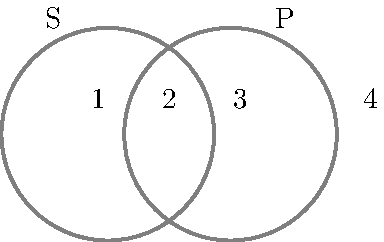
\includepdf[pages=-,pagecommand={},width=\textwidth]{figures/2venn0.pdf}
\end{figure}

\noindent where area 1 represents things that are $S$ but not $P$, area 2 represents things that are both  $S$ and $P$, area 3 represents things that are only $P$, and area 4 represents things that are neither $S$ nor $P$.

Three terms give us eight possibilities to represent, so we draw the diagram like this:

\begin{figure}
\centering
%\begin{syllogism}
%\end{syllogism}
\end{figure}

A four-term sorites will have 16 possible combinations of terms. To represent all of these, we will need to stretch out our circles into ellipses.



The diagram is complex, and it takes some practice to learn to work with it. However, the basic methods for using it are the same as with the three-term diagram. Consider this argument, taken from Lewis Carroll's logic textbook \citep{Dodgson1896}.

\begin{kormanize}
\premise{Nobody who is despised can manage a crocodile.}
\premise{Illogical persons are despised.}
\premise{Babies are illogical.}
\conclusion{No babies can manage a crocodile.}
\end{kormanize}

If we set the major term ``Persons who can manage a crocodile'' as $A$, the minor term ``babies'' as $D$, and the two middle terms as $B$ and $C$, we get this for the Venn diagram.

\begin{description}
\item[$A$:] Persons who can manage a crocodile
\item[$B$:] Persons who are despised
\item[$C$:] Illogical persons
\item[$D$:] Babies
\end{description}
